\chapter{Logbook}

\section{Week 1}

\subsection{30/09/13 - Exploring simple case with PAM modulation}

I received the \emph{PAM.pdf} file outlining the case where a signal is
sent through a channel with AWGN and received with a timing error at the
receiver. I read through the file several times to get an understanding
of the underlying equations.

Leaving the Gram-Charlier series aside for the moment, I started getting
to grips with Mathematica and implementing the transmission system
model:

\[
X = \omega_0 g_0 + \sum_{k=1}^{40} ( \omega_{-k} g_{k} + \omega_k g_k ) + \nu
\]

where $g_k = g((\Delta + k)T)$,
$g(t) = (u_T \ast h_l \ast u_R)(t) \times cos(\theta)$ and $\nu$ is a
zero-mean Gaussian random variate with
$\sigma_{\nu}^2 = N_0 \varepsilon_R$.

I learnt the basics of the interface, and began inplementing the filter
and channel impulse responses (I.R.). I need to double-check the
definition of the Root-Raised Cosine (RRC) Filter, as the impulse
response wasn't as expected.

Later, I found the
\href{http://ntrs.nasa.gov/archive/nasa/casi.ntrs.nasa.gov/20120008631_2012008365.pdf}{correct
form for the RRC} and double-checked it using Octave. The equation used
is listed below. A plot showed that this equation is invalid at
$t = \left [ - \frac{T_s}{ 4 \beta } , 0 , \frac{T_s}{ 4 \beta } \right ]$,
so I plan to find its limit at these points using Mathematica to obtain
the complete solution.

\[
h_{RRC}(t) = \frac{2 \beta}{\pi \sqrt{T_s}} \frac{cos \left [ (1 + \beta) \frac{\pi t}{T_s} \right ] + \dfrac{sin \left [ (1 - \beta) \frac{\pi t}{T_s} \right ]}{\frac{4 \beta t}{T_s}}}{1 - \left ( \frac{4 \beta t}{T_s} \right )^2}
\]

\subsection{01/10/13 - Implementing Raised Cosine functions}

I implemented the function above in Mathematica, and using the
\texttt{Limit} function found the value of the function at the following
undetermined points:

\[
h_{RRC}(t) = \left\{
  \begin{array}{l l}
    \dfrac{4 \beta + \pi (1 - \beta)}{2 \pi \sqrt{T_s}} & t = 0 \\
    \dfrac{\beta}{2 \pi \sqrt{T_s}} \left ( \pi sin \left [ \frac{(1 + \beta) \pi}{4 \beta} \right ] - 2 cos \left [ \frac{(1 + \beta) \pi}{4 \beta} \right ] \right ) & t = \pm \frac{T_s}{ 4 \beta } \\
    \dfrac{2 \beta}{\pi \sqrt{T_s}} \dfrac{cos \left [ (1 + \beta) \frac{\pi t}{T_s} \right ] + \dfrac{sin \left [ (1 - \beta) \frac{\pi t}{T_s} \right ]}{\frac{4 \beta t}{T_s}}}{1 - \left ( \frac{4 \beta t}{T_s} \right )^2} & \text{otherwise}
  \end{array}\right.
\]

I also implemented the Raised Cosine function for the channel function,
using the impulse response below\footnote{Proakis, ``Digital
  Communications''}. I was unable however to convolve the receiver and
transmitter filter functions using the \texttt{Convolve} function, even
when I limited the impulse response using a \texttt{UnitBox}.

\[
h_{RC}(t) = \frac{sinc \left ( \frac{\pi t}{T} \right ) cos \left ( \beta \frac{\pi t}{T} \right )}{1 - \left ( 2 \beta \frac{t}{T} \right )^2}
\]

I looked into Mathematica's treatment of the Gaussian distribution, and
figured out how to generate random noise vectors following a Gaussian
distribution, as well as how to generate a list of random binary
symbols.

After discussing the convolution issue with David, he suggested that the
channel should be initially modelled as ideal and therefore the overall
channel and filter I.R. $g(t)$ can be defined as a Raised Cosine
function, as defined above. I should therefore be ready to implement the
simple ISI model tomorrow.

\subsection{02/10/13 - Wrapping Up the Initial PAM Model}

I pulled together the Raised Cosine function and random number generator
to impiment the given simplified function for the PAM receiver output,
given below. Playing around with the settings, I was able to show how
the $g_k$ function increases with the timing error. I decided to study
the Mathematica environment a little more before carrying on with any
programming.

\[
X = \omega_0 g_0 + \sum_{k=1}^{40} ( \omega_{-k} g_{-k} + \omega_k g_k ) + \nu
\]

\subsection{03/10/13 - Delving deeper into Mathematica}

I devoted some time into looking through Michael Quinlan's notebooks and
better understanding the workings of the \texttt{Table} functions and
the various plotting options. Fortunately my notebook was corrupted so I
was able to rewrite it and understand the model a bit more. I need to
figure out what variance value the noise PDF should take on, as the
noise appears to be overwhelming the timing error effects. Translating
the resulting PDF's into patterns is another question that needs some
thought.

\subsection{Week 1 Summary}

Week 1 was mostly spent becoming acquainted with Mathematica and getting
a feel for the equations underlying PAM transmissions. A simple model of
a PAM receiver was constructed.

\subsection{Goals for Week 2}

\begin{itemize}
\itemsep1pt\parskip0pt\parsep0pt
\item
  The PAM model will need to be extended to calculate the optimum
  decision region boundary from the estimated PDF.
\item
  A better setup will be required to perform large-scale simulations
  within an acceptable time period. We will look into applying for an
  account on the Boole cluster.
\end{itemize}

\section{Week 2}

\subsection{07/10/13 - Matrix manipulations}

I decided to spend another day learning about the Mathematica
environment, in particular matrix manipulation and generation. I looked
into the \texttt{Apply}, \texttt{Map} and \texttt{Partition} functions
and wrote some examples to figure out how to convert mathematical
problems to Mathematica notation using matrices. I hope to convert the
code to use matrices tomorrow to hopefully simplify and speed things up.

I also implemented David's equation for properly calculating the AWGN
function variance from SNR\footnote{See \emph{davenotes.pdf}}, from last
Friday's meeting.

\subsection{08/10/13 - Fixed I.R. and Kernel Density Estimation}

The first job was to rewrite the code to make use of the simple dot
operator to calculate all the ISI components\footnote{The ISI components
  are now calculated using: \[
  \left [
    \sum_{k=0}^{k=40} \left ( g_k \omega_k^j + g_{-k} \omega_{-k}^j \right ) \cdots
  \right ]^{j=\{1..m\}} = \\
\left [ 
    g_{-40} \cdots g_{-1} g_{1} \cdots g_{40}
  \right ] \bullet \left [
    \begin{matrix}
  \omega_{-40}^j  \\
  \vdots          \\
  \omega_{-1}^j   \\
  \omega_{1}^j     \\
  \vdots            \\
  \omega_{40}^j    \\
    \end{matrix}
  \right ]^{j=\{1..m\}}
  \] where $\omega_{k}^j$ is the $k$'th ISI with the $j$'th timing
  offset.}. With the new code I was able to carry out many more runs and
get much more detailed output. In addition, when I was rewriting the
code I noticed a typo in the Raised Cosine I.R. that was degrading
performance in the perfectly synchronised case. With both of these
changes made, I decided to use Kernel Density Estimation to see what
effects the timing offset has.

Using offsets of 10\textsuperscript{-15}, 0.05, 0.1 \& 0.15, the
following values of $g_k, k \in \{ -40 \dots -1, 1 \dots 40 \}$ were
calculated.

\begin{figure}[htbp]
\centering
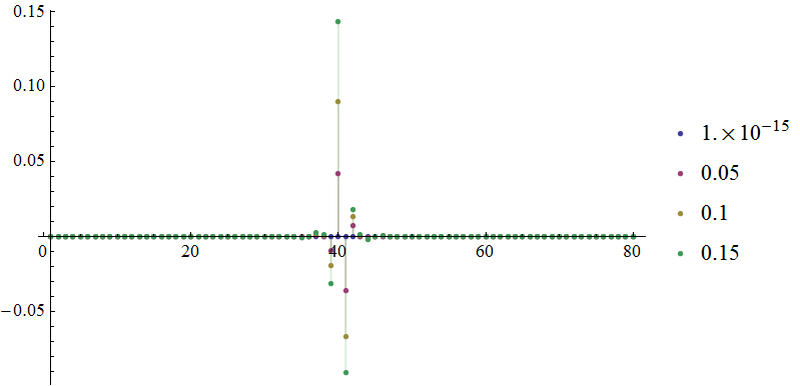
\includegraphics[width=\linewidth]{../../../plots/fyp1_w1_gklin.png}
\caption{$g_k$ linear plot}
\end{figure}

\begin{figure}[htbp]
\centering
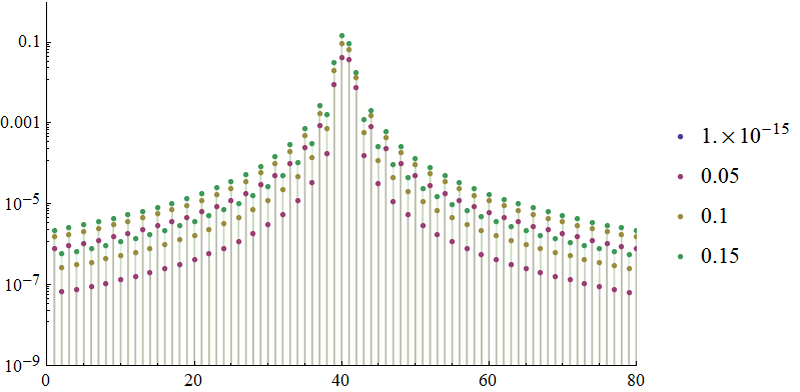
\includegraphics[width=\linewidth]{../../../plots/fyp1_w1_gklog.png}
\caption{$g_k$ log plot}
\end{figure}

Using \texttt{SmoothKernelDistribution} to perform Kernel Density
Enstimation with 1 million points produced the following estimated PDFs
for both possible transmitted values. As the timing error increases, we
note that the PDF spreads out, but the mean remains steady.

\begin{figure}[htbp]
\centering
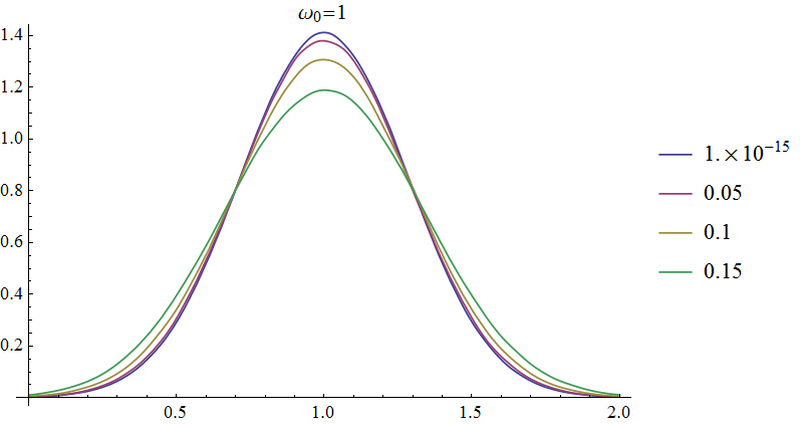
\includegraphics[width=\linewidth]{../../../plots/fyp1_w1_kde.png}
\caption{kernel density estimation $\omega_0=1$}
\end{figure}

\begin{figure}[htbp]
\centering
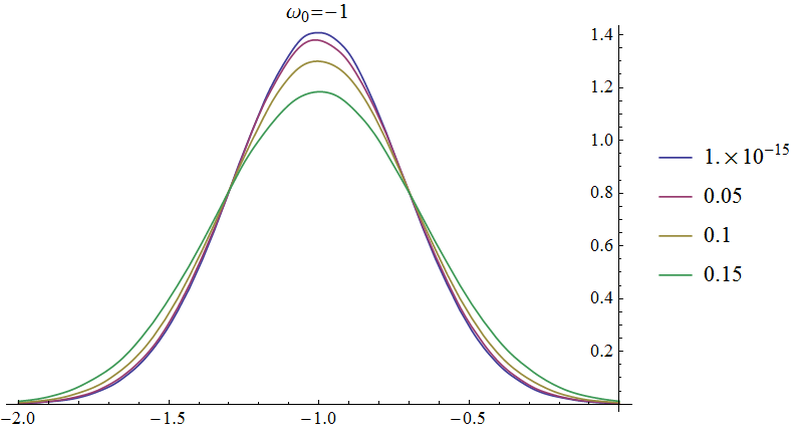
\includegraphics[width=\linewidth]{../../../plots/fyp1_w0_kde.png}
\caption{kernel density estimation $\omega_0=-1$}
\end{figure}

\subsection{09/10/13 - Setting up Digital Comms Lab PC}

With Ger's help, I set up an account on \texttt{Digital Comms Lab 1} \&
\texttt{Digital Comms Lab 2} and got the internet working. Mathematica 8
is installed and working on both machines, we will have to consider
whether an upgrade to Mathematica 9 would be useful or not. Git and VNC
or similar have to be installed next. A request was made to the Boole
cluster for access for this machine, however the email given
(\texttt{bcrisupport@bcri.ucc.ie}) was invalid.

\subsection{10/10/13 - Probing the Elec Eng network}

After finding out the Boole cluster was no more, I used today to examine
what hardware I had available to me. I got access from Ger to the public
\texttt{UEPC004} server, and from there I am able to access machines on
the elec eng network. I set up a \emph{Remote Desktop Protocol} link to
\texttt{Digital Comms Lab 1} through this server, allowing me to control
the machine from any location. I am also able to log remotely into EDA
lab machines, and run Mathematica 6 on those machines.\footnote{The GUI
  does not work when using \texttt{ssh} to access the EDA Lab machines,
  but using the command \texttt{math} to start and operate Mathematica
  kernels does.} Ger has been known to tweak machines in response to
personal requests, so if asked nicely he may let me use two or three of
these machines concurrently.

Given these resources, I feel there are three ways I could continue:

\begin{itemize}
\itemsep1pt\parskip0pt\parsep0pt
\item
  I could upgrade to the latest version of Mathematica on all machines,
  and set up a Mathematica cluster with \texttt{Digital Comms Lab 1} as
  the front end and the EDA Lab PCs as remote nodes. With this setup,
  all machines would act as one (as in a traditional cluster). This
  would be the easiest to use, but would require considerate work to set
  up.
\item
  I could use the \texttt{MathLink} interface to acheive a similar,
  lower-level version of the former, with the EDA Lab machines as
  independent, remote slaves and \texttt{Digital Comms Lab 1} sending
  commands to these slaves and collating the replies. This setup is
  distributed computing with a star topology, and would be easier to
  setup. The downside is that the code needs to manually divide the task
  between each of the nodes, and needs to be well designed to minimise
  network delays.
\item
  I could simply run the code in parralel on each of the machines
  available to me, dumping the results to text files, and collate the
  data at the end. This would require no setup, and code written on any
  machine would only require porting to another version of Mathematica.
  Additionally this seems like it would deal best with hiccups such as
  machines going down and it does not depend on a connection between the
  machines. The downside is there would be some overhead with collecting
  the results afterwards.
\end{itemize}

\subsection{Week 2 Summary}

I fixed the code written last week and began setting up my simulation
environment.

\subsection{Goals for Week 3}

\begin{itemize}
\itemsep1pt\parskip0pt\parsep0pt
\item
  Work out a setup that will allow me to carry out largeer-scale
  simulations.
\item
  Adapt the previous code to run in parallel and produce useful
  machine-readable output.
\end{itemize}

\section{Week 3}

\subsection{14/10/13 - Running longer scripts on the EDA machines}

Today I spent some time figuring out how to build and run scripts on the
EDA machines. I found that defining a module in a text file and copying
the Mathematica code into the module allows the code to be called with
input arguments, and writing the output to a text file and placing the
module in a loop allows each pass to be recorded for later
parsing\footnote{Using the \texttt{Get} and \texttt{Put} methods. The
  \texttt{DumpSave} method is supposed to be more efficient, but was
  added after Mathematica 6.}. After running the code overnight, this
system appears to work, and is scaleable over multiple machines. The
main disadvantage is the size of these files (7.7MB per 400,000 values),
so I must either figure out how to transfer them over the network or see
whether reducing the precision of the output values will reduce the file
sizes.

\subsection{15/10/13 - Reducing output size}

Given the 15GB of samples produced the night before was far too much to
pull off the machine, I copied 20 million of the samples and plotted
them to make sure the script had worked in practice\footnote{For the
  record, I could only use a fraction of them, as loading all 20 million
  samples crashed the machine for over an hour.}. I then looked into how
I could reduce the size of the output produced, and decided to replace
the \texttt{SmoothKernelDistribution} function (which came in after
Mathematica 6.0 and therefore couldn't be used on the EDA machines) with
a fine-grained histogram function\footnote{I am assuming that both
  approach the true PDF as $\text{N} \! \rightarrow \! \infty$}. This
allowed me to add the probabilities generated in each sweep to those
generated before and keep the output to a handful of 1kB files. I ran
the simulation overnight to check it.

\subsection{16/10/13 - Moving onto 4-PAM}

Checking the output from the night before, I get a similar PDF plot as
with the \texttt{SmoothKernelDistribution} function. I therefore
modified the code to examine all 3 decision region boundaries in a 4-PAM
system and ran the simulation for 100 million samples per condition. The
resulting distributions shown below show increased probability of error
with timing error, as expected, but decision region boundaries in this
case remain the same.

\begin{figure}[htbp]
\centering
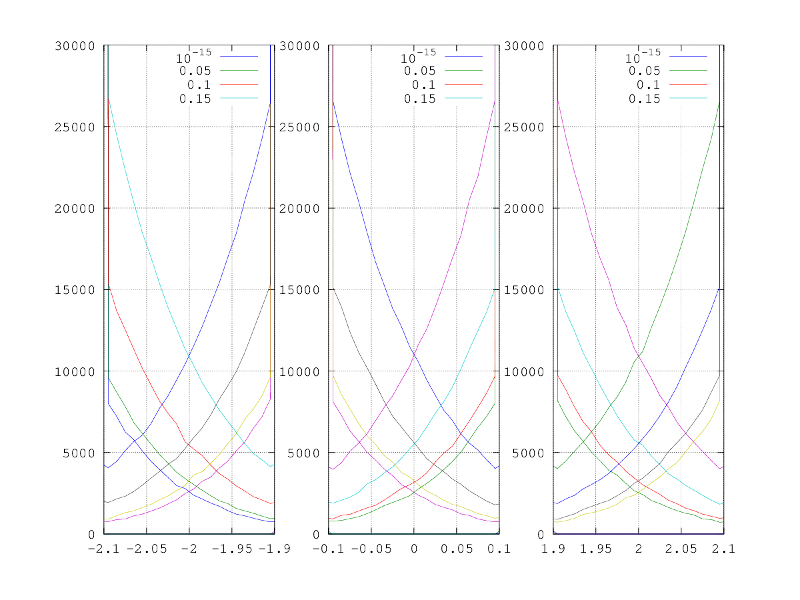
\includegraphics[width=\linewidth]{../../../plots/4pamdecision.png}
\caption{PDF for 4-PAM, $\omega_0 \in {-3,-1,1,2}$, $10^8$ samples}
\end{figure}

I could imagine finding a value for the probability of error and moving
onto PSK systems as the next steps in the process.

\subsection{Week 3 Summary}

Code was written that could be executed in parallel on multiple
machines, and this was demonstrated in practice. The code was extended
to the 4-PAM case, and showed no change in optimum decision region
boundaries. Upon later consultation with Dave, it seems this is because
the decision region boundaries shift due to a change in the $g_0$ term,
and not the appearance of ISI components due to the $g_k$ terms; the
latter was believed to be the expected cause, and so the $g_0$ term was
assumed to be 1 in the code.

\subsection{Goals for Week 4}

\begin{itemize}
\itemsep1pt\parskip0pt\parsep0pt
\item
  Re-run the simulations to see if implementing the change in $g_0$ with
  timing error changes the location of the optimum decision region
  boundaries.
\item
  If so, it would be interesting to see if the Gram-Charlier
  approximation produces the same boundary locations.
\end{itemize}

\section{Week 4}

\subsection{21/10/13 - Implementing the Gram-Charlier series}

Over the weekend, I implemented the $g_0$ term fix discussed in our
Friday weekly meeting and re-ran the simulation, this time across two
machines. Results showed that the Decision Region Boundary is displaced
towards the origin as the timing offset increases.

\begin{figure}[htbp]
\centering
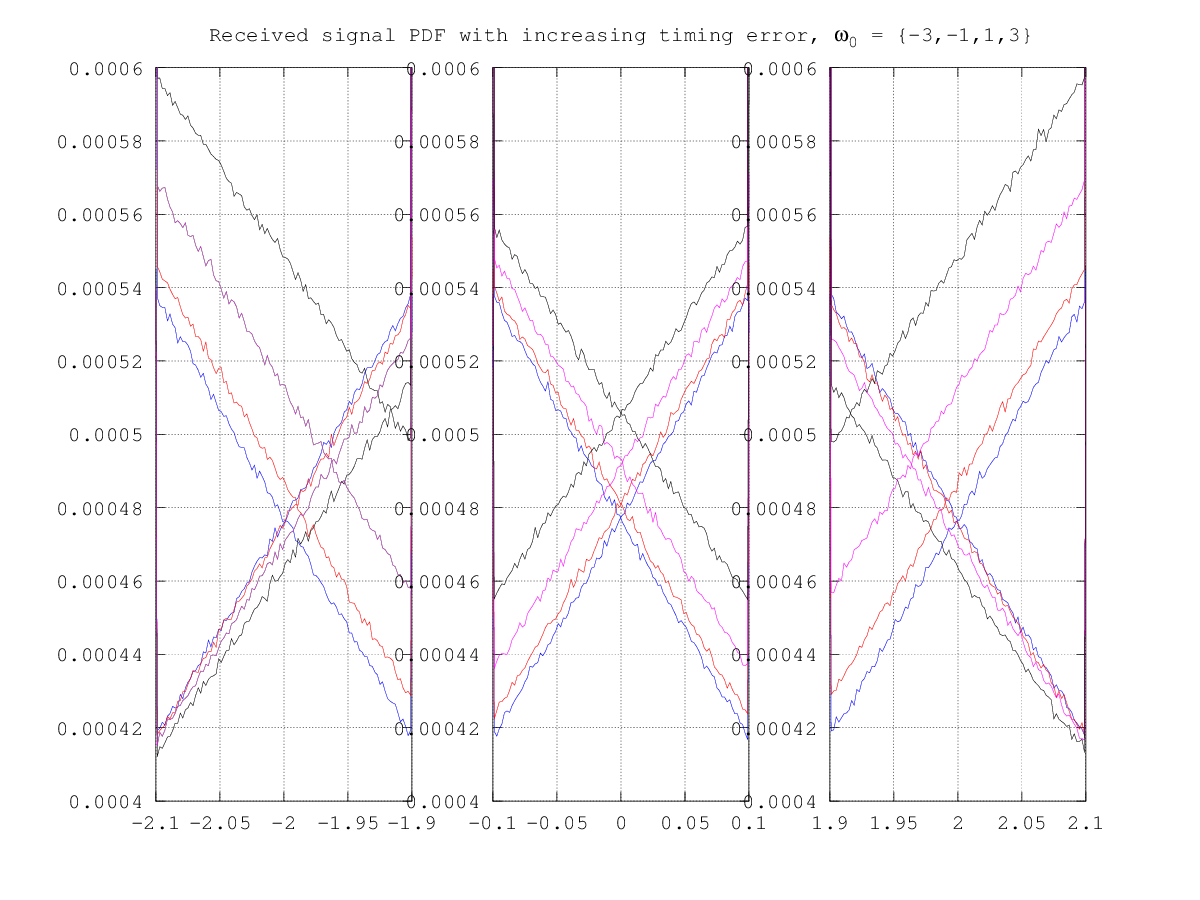
\includegraphics[width=\linewidth]{../../../plots/4pamdecisionerror.png}
\caption{PDF for 4-PAM, $\omega_0 \in {-3,-1,1,2}$}
\end{figure}

I spent Monday carrying out two tasks:

\begin{enumerate}
\def\labelenumi{\arabic{enumi}.}
\itemsep1pt\parskip0pt\parsep0pt
\item
  I re-wrote Dave's Gram-Charlier equations\footnote{See
    \emph{davenotes.pdf}} for Mathematica, and should be ready to try
  them out tomorrow.
\item
  I modified the PAM simulation with a coarser-grained histogram, but
  more timing offset values, in order to see how the decision variate
  varies with timing offset. The results should be available in the
  morning.
\end{enumerate}

\subsection{22/10/13 - More Gram-Charlier series}

The simulation results showed that the decision region boundaries did
decrease with timing error, however the histogram was not fine-grained
enough to accurately determine the exact boundary locations, so the
simulation was re-run with more bins.

I fixed some bugs in my implementation of the Gram-Charlier series and
was able to generate a few plots, which were very similar to those
generated by the simulator, albeit with half the amplitude. A goal for
tomorrow is to generate the plots with identical timing offsets to the
simulation and compare both plots.

\subsection{23/10/13 - Proper Gram-Charlier plots}

The simulation results had been appended to the previous set of results
by accident, so the whole thing had to be run again for tomorrow. On a
more positive note, I noticed a missing power in my implementation of
the Gram-Charlier series, and the plots are now a lot closer to those
generated previously.

\subsection{Week 4 Summary}

I implemented the Gram-Charlier series and was able to compare the
results from the simulationa dn the Gram-Charlier series. These are
close, but not exact, so we will have to look closely at where the
differences may be coming from.

\subsection{Goals for Week 5}

\begin{itemize}
\itemsep1pt\parskip0pt\parsep0pt
\item
  I will make use of the long weekend to run some extra-long simulations
  and compare these to the Gram-Charlier series.
\end{itemize}

\section{Week 5}

\subsection{29/10/13 - Comparing Gram-Charlier to Simulation}

The simulations ended, and I was able to compare simulated and
gram-charlier PDF plots. I extracted a rough estimate of the decision
region boundaries given by both methods and compared them to the
corresponding values of $2 g(\Delta)$, and found very close correlation.

\begin{figure}[htbp]
\centering
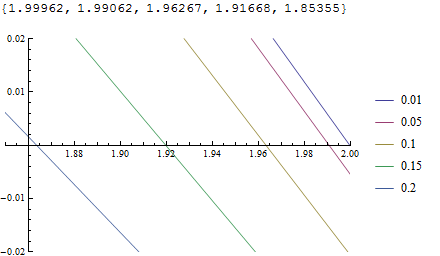
\includegraphics[width=\linewidth]{../../../plots/gcdrb.png}
\caption{Gram Charlier approximation of
$P(\omega_0=1,R)-P(\omega_0=3,R)$}
\end{figure}

\begin{figure}[htbp]
\centering
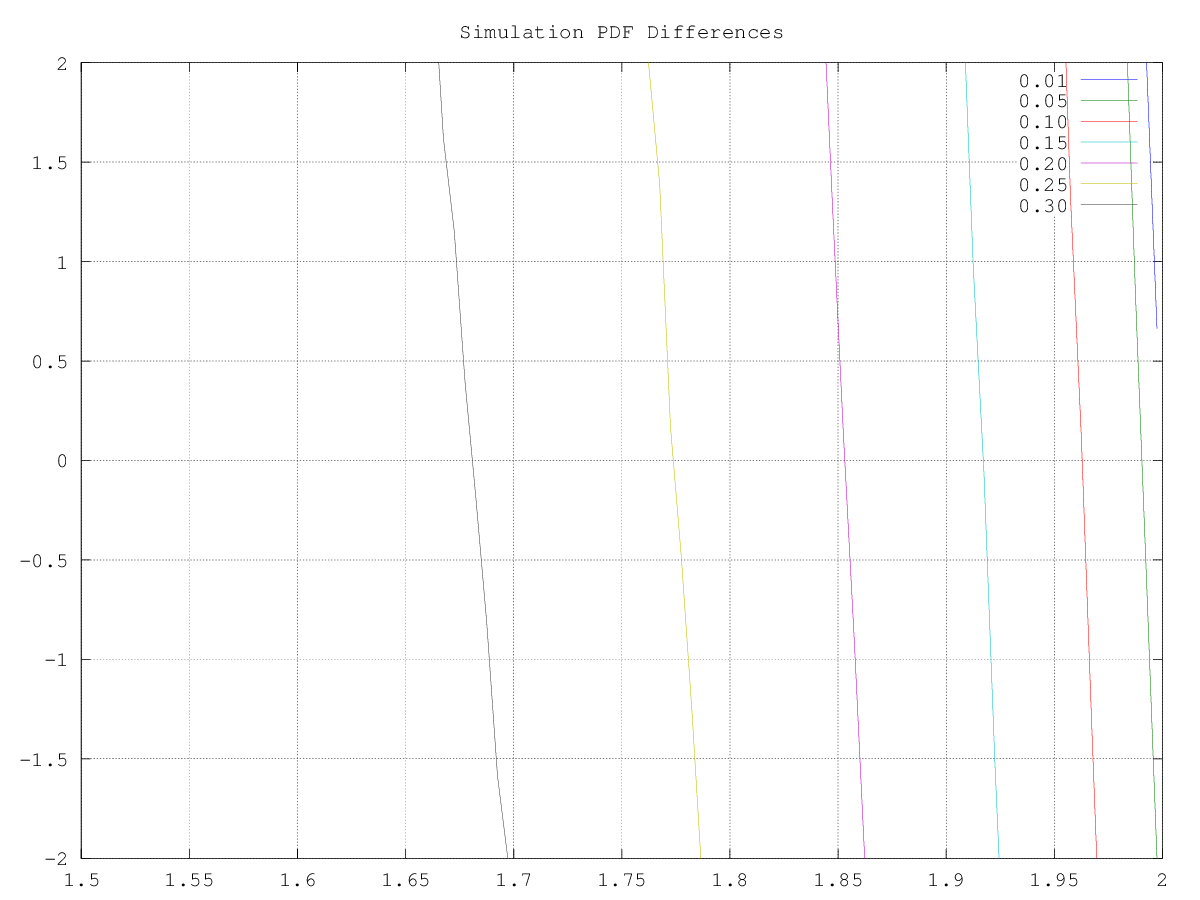
\includegraphics[width=\linewidth]{../../../plots/simdrb.png}
\caption{Simulation of $P(\omega_0=1,R)-P(\omega_0=3,R)$,
N=$3 \times 10^6$}
\end{figure}

\begin{figure}[htbp]
\centering
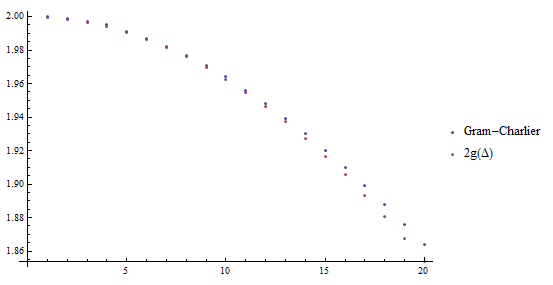
\includegraphics[width=\linewidth]{../../../plots/gc_vs_2g.png}
\caption{Comparison of Gram-Charlier Decision Region Boundaries and
$2 g(\Delta)$ estimation ($0.01 \ge \Delta \ge 0.2$)}
\end{figure}

\subsection{30/10/13 - Applying the Tikhonov Distribution}

I was able to implement the Tikhonov Distribution using the equation
provided in \emph{PAMTikhonov.pdf}:

\[
F_{\Delta} (y) = \frac{\text{Exp}\left [ \dfrac{cos(2 \pi y)}{(2 \pi \sigma_{\Delta})^2} \right ]}{I_0 \left ( \dfrac{1}{(2 \pi \sigma_{\Delta})^2} \right )} \text{  where  } -\frac{1}{2} \le y \le \frac{1}{2}
\]

Given these timing error probabilities and the optimum decision region
boundaries for each timing error, I calculated the overall optimum
decision region boundary for each timing error probability distribution
using

\[
B_{\text{OPT}} \sim \sum_{\Delta} \text{P}(\Delta) B_{\text{OPT,}\Delta}
\]

\begin{figure}[htbp]
\centering
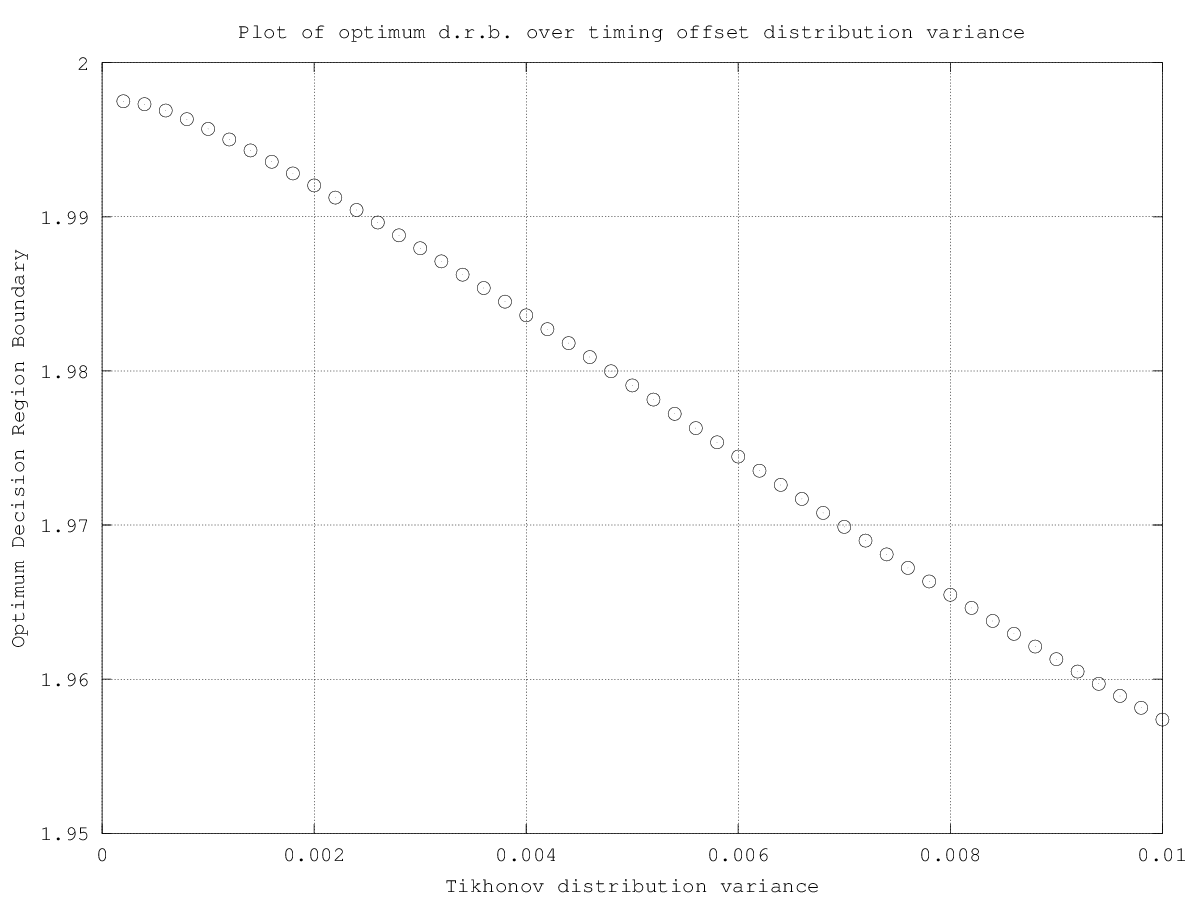
\includegraphics[width=\linewidth]{../../../plots/odrb_vs_tikhvar.png}
\caption{Optimum Decision Region Boundary for various timing error
probability distributions}
\end{figure}

It is important to note that with increasing variance, the probability
density function places more weight on larger timing errors outside the
range simulated, so these results are less accurate for higher
variances.

\subsection{Week 5 Summary}

In week 5, I calculated the optimum decision region boundary for a range
of timing offsets, through simulation and the Gram-Charlier
approximation. I demonstrated a close correlation between these
boundaries and the $2 g_k$ term. A slight difference between the
Gram-Charlier approximation was found to be due to a typo in its
implementation. I applied the Tikhonov distribution to the calculated
optimum decision region boundaries for each timing offset, in order to
calculate an optimum decision region boundary for a given Tikhonov
distribution of timing offsets

\subsection{Goals for Week 6}

\begin{itemize}
\itemsep1pt\parskip0pt\parsep0pt
\item
  On the simulation side, a key goal for week 6 is to randomly generate
  timing offsets according to the Tikhonov distribution and apply these
  to the simulation as timing offsets, in order to verify correlation
  with the Gram-Charlier and $2 g_k$ approximations.
\item
  A typo in the Gram-Charlier implementation has been found and
  corrected, and it would be interesting to see if this approximation
  matches $2 g_k$.
\end{itemize}

\section{Week 6}

\subsection{04/11/13 - Fixing errors}

Dave took a look at my code and spotted errors which I fixed. The fixed
Gram-Charlier implementation was found to match $2 g_k$ very closely.
The fixed simulation was left to run overnight; unfortunately
Mathematica 6.0 running on the Unix machines was unable to run it, so
the number of points had to be reduced.

\subsection{05/11/13 - Corrected simulation results}

The produced PDFs were too inaccurate to properly calculate the zero
crossing points, so the simulation will have to be run over several
days.

\subsection{Week 6 Summary}

A simulation was constructed that generated timing error offsets
according to a Tikhonov distribution of predetermined variance, and used
to produce received symbol PDFs. The simulation was found to run very
slowly, and could only be run on Mathematica 9. Ger has been asked
whether it would be possible to upgrade the Unix machines to this
version and he will look into it.

\subsection{Goals for Week 7}

\begin{itemize}
\itemsep1pt\parskip0pt\parsep0pt
\item
  Continue running the simulation, trying to speed it up if at all
  possible.
\end{itemize}

\section{Week 7}

\subsection{11/11/13 - Returning to the UNIX machines}

The UNIX machines were upgraded to Mathematica 9 over the weekend, so I
was able to port the code in order to run off these. In addition, Dave
suggested that I look into parralising the code. Since these were
dual-core machines I was able to make use of Mathematica's
\texttt{ParallelTable} function to reduce run times a little. Th
simulation will have to run over several days, however, as the expected
deviation in optimum decision region boundary is very small.

\subsection{19/11/13 - Day 9 of Week 7}

After several days of running the simulations, we found the optimum
decision region boundaries given by the simulations, in red, converged
to roughly those predicted by averaging the optimum decision region
boundary of a timing offset over the tikhonov distribution of timing
offsets, in blue, given by the equation:

\[
B_{\text{OPT}} \sim \sum_{\Delta} \text{P}(\Delta) B_{\text{OPT,}\Delta}
\]

\begin{figure}[htbp]
\centering
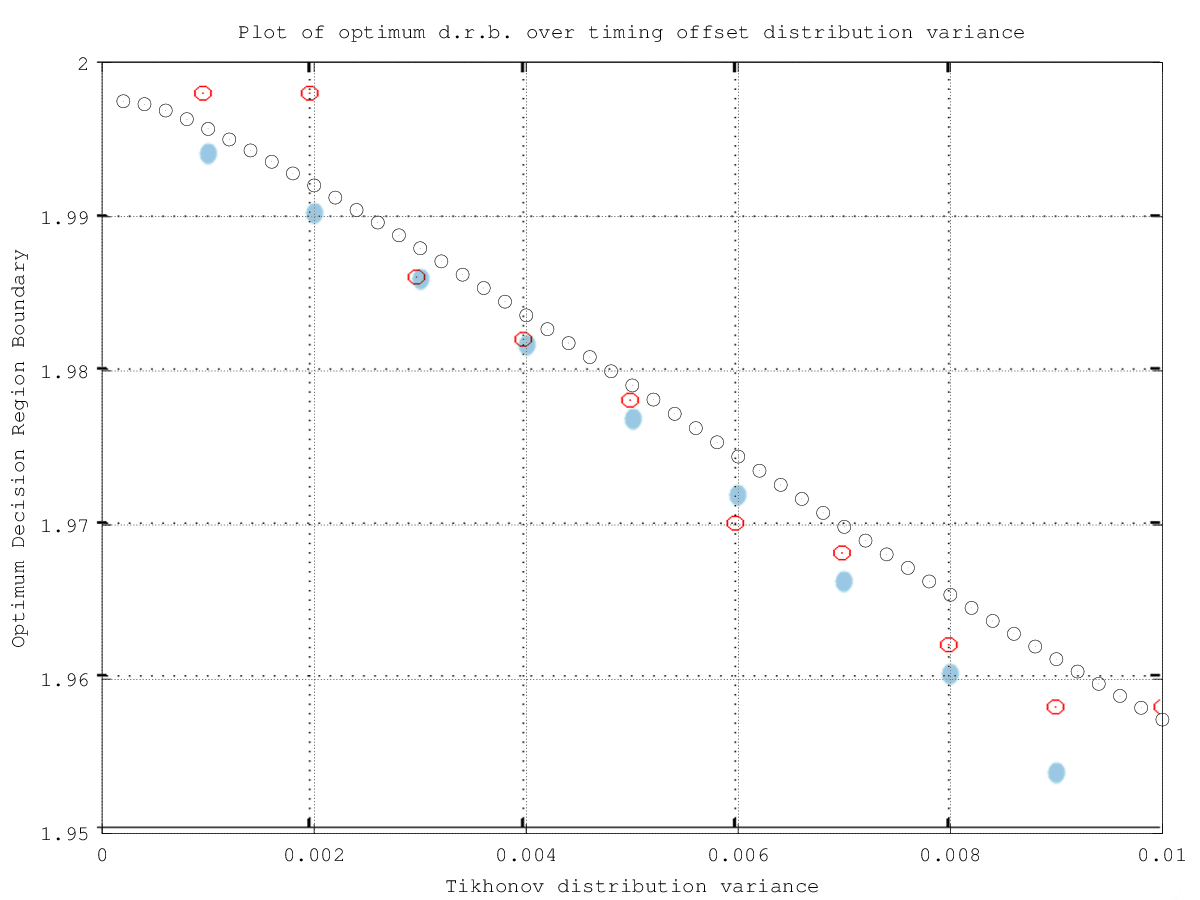
\includegraphics[width=\linewidth]{../../../plots/opt_dec_reg.png}
\caption{Optimum Decision Region Boundary for various timing error
probability distributions. Black: estimate found by averaging fixed timing errors over Tikhonov distribution; Blue: analytical result determined by Dave; Red: simulation results.}
\end{figure}

\subsection{Week 7 Summary}

Simulations supported the theory that the optimum decision region
boundary in the presence of statistically distributed receiver timing
errors will decrease from the expected value. Additionally, it was shown
through simulation that the new optimum decision region boundary can be
aproximated, assuming a known distribution of these timing errors, by
averaging the optimum decision region boundary given each timing offset
over the distribution of timing offsets.

\subsection{Goals for Week 8 onwards}

\begin{itemize}
\itemsep1pt\parskip0pt\parsep0pt
\item
  Verify that the Gram-Charlier series provides an adequate
  approximation to the received symbol PDF in the presence of timing
  errors.
\item
  Provide numerical values for the probability of error $P_e$ in the
  presence of a distribution of timing errors.
\end{itemize}

\section{Week 8}

Additional simulation was carried out in order to provide a more accurate representation of the received signal PDF. Work on the preliminary report was also started.